\section*{Overview}

Centroid decomposition is the tree technique I use when path information is global but still structured enough that one
balanced separator can expose it. It repeatedly splits the tree at a centroid, producing a recursion tree of depth
\(O(\log n)\).

\section*{When to Use It}

Use centroid decomposition when:

\begin{itemize}
  \item the graph is a tree,
  \item the query or counting logic depends on paths,
  \item processing all paths through one special vertex is manageable,
  \item rerooting or heavy-light decomposition does not match the query pattern directly.
\end{itemize}

Typical examples include nearest marked node, counting paths with a distance constraint, and subtree-independent path
aggregation.

\section*{Core Idea}

A centroid of a tree is a vertex whose removal leaves no component larger than half of the current tree. If I recurse on
the remaining components after removing that centroid, every original vertex participates in only \(O(\log n)\) levels
of the decomposition.

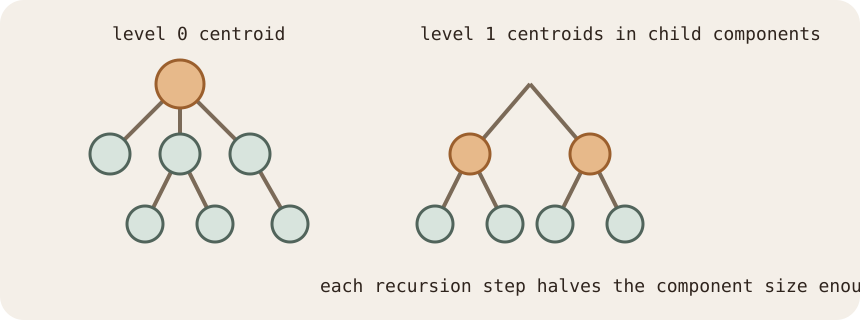
\includegraphics[width=\textwidth]{figures/centroid-layers.svg}

\section*{Key Insight}

Every path in the original tree passes through the centroid of some decomposition component. That is the structural
reason the method works: if I know how to process all paths passing through the current centroid, recursion takes care of
the paths that stay entirely inside one child component.

\section*{Operations / Main Technique}

\begin{itemize}
  \item compute subtree sizes,
  \item find the centroid of the current component,
  \item process the path information that uses this centroid,
  \item remove it logically and recurse on each remaining component.
\end{itemize}

\paragraph{Worked example.}
For nearest-red-node queries, each node stores its chain of centroid ancestors and the distance to each of them. Updating
one red node touches only those ancestors, and querying another node checks the same ancestor chain.

\section*{Correctness Intuition}

The recursion is complete because every path either passes through the current centroid or lies entirely inside one
remaining component after the centroid is removed. Those two cases are disjoint, so processing them separately covers
all paths exactly once at the right recursion level.

\section*{Complexity Analysis}

Centroid decomposition builds in \(O(n \log n)\) total time for the standard adjacency-list implementation. Many query
schemes layered on top of it become \(O(\log n)\) or \(O(\log^2 n)\) per update/query.

\section*{Implementation}

The code builds the centroid parent tree and records the decomposition depth of each node. That is the reusable core I
want before specializing to one particular path problem.

\section*{Common Pitfalls}

\begin{itemize}
  \item Forgetting that the processing work per centroid still decides whether the full solution is fast enough.
  \item Mutating the original tree structure in a way that breaks later recursion.
  \item Mixing the original tree parent with the centroid-tree parent.
  \item Using centroid decomposition for simple subtree-only queries that Euler tour already solves cleanly.
\end{itemize}

\section*{Variants / Extensions}

\begin{itemize}
  \item Nearest active node queries.
  \item Count or optimize over paths with bounded length or weighted constraints.
  \item Combine with LCA distance queries or precomputed depth arrays.
\end{itemize}

\section*{Practice Problems}

\begin{itemize}
  \item Xenia and Tree style nearest-marked-node queries.
  \item Count paths whose length or weight satisfies a condition.
  \item Recursively process tree paths through balanced separators.
\end{itemize}

\section*{References}

\begin{itemize}
  \item \href{https://cp-algorithms.com/graph/centroid_decomposition.html}{cp-algorithms: Centroid Decomposition}.
  \item \href{https://usaco.guide/plat/centroid?lang=java}{USACO Guide: Centroid Decomposition}.
  \item \href{https://codeforces.com/catalog?locale=en}{Codeforces Catalog}.
\end{itemize}
